\chapter{Eulerian Domain: Finite Element Method}
\label{ch:eulerian}
	\lsymb[f]{$\mathcal{T}_h$}{Finite Element mesh}{-}{th}		
	\lsymb[f]{$T$}{Cell of Finite Element mesh}{-}{t}			
	
	\lsymb[f]{$v$}{Test function}{-}{v}				
	\lsymb[f]{$V$}{Trial vector function space}{-}{vte}				
	\lsymb[f]{$\hat{V}$}{Test vector function space}{-}{vtr}					
	\gsymb[f]{$\Omega$}{Fluid domain}{-}{x}	
	\gsymb[f]{$\Omega_E$}{Eulerian fluid domain}{-}{xe}	
	\gsymb[f]{$\Omega_L$}{Lagrangian fluid domain}{-}{xl}	
	\gsymb[f]{$\partial \Omega$}{Boundary of the domain $\Omega$}{-}{xdd}	

%------------------------------------------------------------------------------------------------------
%------------------------------------------------------------------------------------------------------
%------------------------------------------------------------------------------------------------------
%\section{Purpose of eulerian domain}
Standard \printAcron{Computation Fluid Dynamics}{CFD} method discretizes the fluid into smaller regions, known as grids, and solves the set of Navier-Stokes equations in this region. This type of formulation is referred to as an Eulerian method, as we are evaluating the change of flow property in a given volume.

For the hybrid method, we use the Navier-Stokes grid formulation in the near-body region. The advantage of using the Eulerian method at this region is that it is much more efficient in resolving the boundary layer than the Vortex Particle Method. We can directly enforce the wall boundary condition at the wall boundary of the Eulerian domain, solving the problem of vorticity generation of the body. In the hybrid coupling strategy, we can then interpolate this newly resolved near-wall solution on to the Lagrangian domain, where the vortex blobs can efficiently evolve the particles.

The various approaches to solve the fluid dynamics problem from a Eulerian reference frame. \indexAcron{Finite Volume Method }{FVM}, \indexAcron{Finite Difference Method}{FDM}, and \indexAcron{Finite Element Method}{FEM} are the common choice for solving the Navier-Stokes problem and differ by the way they approach to solve the problem. FVM divides the domain into volumes where it enforces the conservation of mass and momentum in each sub-domains. FDM divides the domain into nodes and use local Taylor expansions to approximate the partial differential equations. FEM divides the domain into elements and solves the problem using variational calculus. So in the end, the choice of Eulerian method does not have a direct impact on the coupling with the Lagrangian method as the purpose of the Eulerian method is only to efficiently, and accurately resolve the near-body region of the body.

We have decided to use the FEM packages provided by the \fenics project as they have be already implemented efficient, multi-threaded algorithms for solving the partial differential equation. Furthermore, they provide extensive features for future developments such as adaptive mesh refinement, fluid-structure interaction, and efficient computation of turbulent flow.

\section{Introduction to Finite Element Method}

\printAcron{Finite Element Method}{FEM} is numerical method to solve for the solution of a given partial differential equation. It is solved by describing it as a variation problem, giving us an approximate solution for the boundary value problem \cite{Brenner2002}. So the FEM approximates the unknown variables and converts the partial differential equations to a set of algebraic equations, which makes them easier to solve. It was traditionally used for solid mechanics (e.g for the analysis of aircraft structures \cite{RAO2011}), but have since then used to solve fluid dynamics problems \cite{Guermond2006a} \cite{Johnston2004a} \cite{Guermond2003a}.

\subsection*{Finite element discretization}

The finite element solves problem by dividing the domain of interest into smaller, simpler regions known as ``elements". These ``elements" are connected at the joints which are called nodes or nodal points. We use these sets of node and elements to represent the actual variation in the field (such as the displacement, the velocity, the pressure or the temperature) using simple functions, known as the basis functions. Thus, we have transformed the domain of interest into finite number of \indexAcron{Degrees of Freedom}{DOF}. We combine the set of equations of the element into a global system of equations to solve for the unknown.

	\begin{figure}[b]
	\centering
	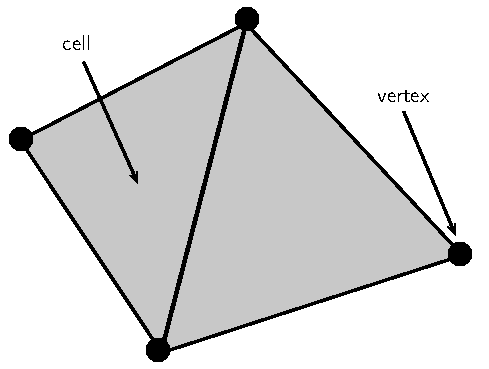
\includegraphics[width=0.4\linewidth]{./figures/eulerian/finiteElementDefinitions.pdf}
	\caption{A two-dimensional finite element geometry. The cell represents the area of the element, and vertices are the edges of the cell.}
	\label{fig:finiteElementDefinitions}
	\end{figure}

A finite element discretization in 2-D can be seen in figure \ref{fig:finiteElementDefinitions}. The figures shows two connected elements, where the cells represent the area of the element, and the vertices of the cell represents the nodes of the element. The finite number of cells $\mathcal{T}_h = \{T\}$ of the fluid domain $\Omega$, together makes the mesh of the Eulerian domain. As shown in figure \ref{fig:finiteElementDefinitions}, the cells of the finite element in 2-D, are made of simple geometrical shapes such as triangles or quadrilaterals. There are two approaches to discretize the domain: structured or unstructured mesh. The structured mesh has cells oriented in a structured pattern, and is the simplest approach in discretizing the mesh. The advantage of such a discretization is that it is possible to make a simple data structure which can be used to perform efficient computation. The downside to such discretization is that the mesh quality deteriorates as one increases the complexity of the domain. However, the FEM enables us to perform an unstructured discretization of the domain, as shown in figure \ref{fig:cylinderFiniteElementDiscretization}. The figure shows the unstructured discretization of the fluid domain around the cylinder $\Omega_E$, connecting the rectangular outer boundary of the fluid to the circular no-slip boundary of the body in a simple fashion. This shows that even though the unstructured method formulation is more complicated that the structured formulation, we have the advantage that the mesh quality does not deteriorate as the domain becomes more complex.

There are several algorithms for mesh generation. The standard approach is to employ the Delaunay triangulation method derived from the Voronoi diagram concept \cite{Carey1997}. This divides the domain into a set of triangles, as shown in figure \ref{fig:cylinderFiniteElementDiscretization}. This type of mesh generation allows us to connect different shapes of boundary with each other. Furthermore, this triangulation method be controlled by predefining the boundary element nodes using a transfinite interpolation.

\begin{figure}[t]
        \centering
        \begin{subfigure}[b]{0.5\textwidth}
                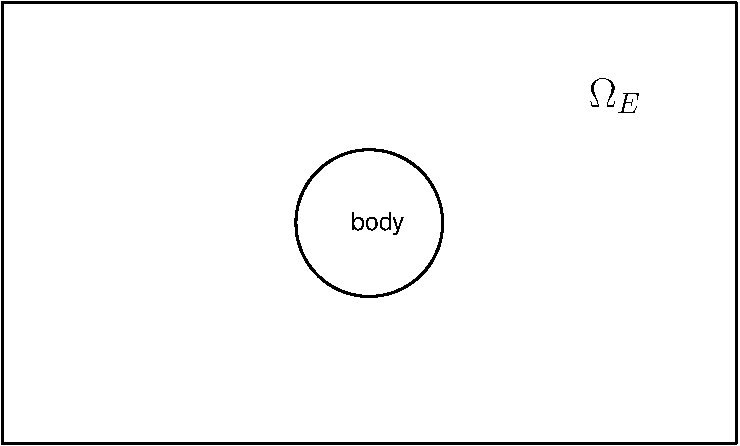
\includegraphics[width=\textwidth]{figures/eulerian/cylinderPreDelauney-crop.pdf}
                \caption{Fluid domain $\Omega_E$ around the cylinder}
                \label{fig:cylinderPreDelauney}
        \end{subfigure}%
        ~ %add desired spacing between images, e. g. ~, \quad, \qquad etc.
          %(or a blank line to force the subfigure onto a new line)
        \begin{subfigure}[b]{0.5\textwidth}
                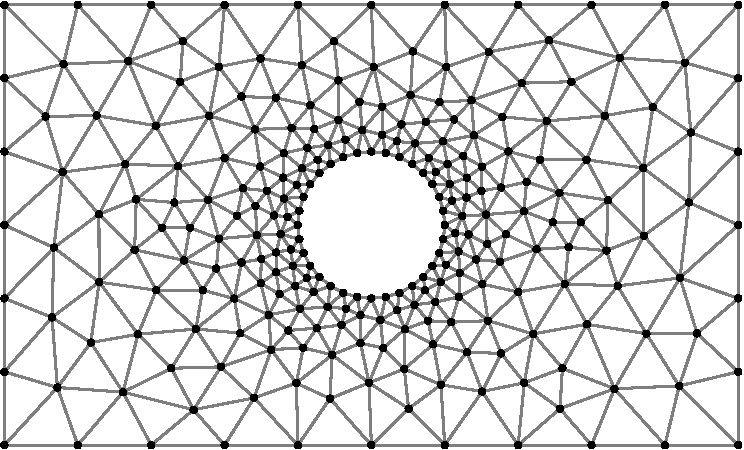
\includegraphics[width=\textwidth]{figures/eulerian/cylinderDelauney-crop.pdf}
                \caption{Delaunay triangulation of the fluid}
                \label{fig:cylinderDelauney}
        \end{subfigure}
        \caption{Delaunay triangulation of the fluid around a cylinder resulting in unstructured mesh with controllable cell sizes.}
        \label{fig:cylinderFiniteElementDiscretization}
\end{figure}	

\subsection*{Finite element function and function space}

The finite element is defined using a triple ($T, \mathcal{V}, \mathcal{L}$), as defined Ciarlet \cite{Ciarlet1972b} and used by the \fenics Project \cite{Logg2012b}. The domain $\Omega$ is divided into cells $T$, the space $\mathcal{V} = \mathcal{V}(T)$ is a finite dimensional function space on $T$ of dimension $n$, and $\mathcal{L} = \left\{ \ell_1,\ell_2,...,\ell_n \right\}$ is the set of degrees of freedom forming the basis for the dual space $\mathcal{V}'$ of $\mathcal{V}$.

When the domain $\Omega$ is divided into cells $T$, we can define the function and the function space of the finite element problem. For each cell, a local function space $\mathcal{V}$ can be defined to collectively construct the global function space $V$. Any given function $u \in V$ is a expressed in a linear combination of basis functions $\{\phi_1,\phi_2,...,\phi_N\}$,  of the function space $V$, 
	\begin{equation}
	u(x) = \sum_{j=1}^N U_j\phi_j(x).
	\end{equation}

There are several types of finite element families: the Brezzi-Douglas-Marini, the Crouzeiz-Raviart, the Discontinuous Lagrange, the Hermite, and the Lagrange elements \cite{Logg2012b}. Each has its own advantage such as the Discontinous Lagrange, or \indexAcron{Discontinous Galerkin}{DG} element consists of discontinuous functions, which was originally introduced for solving hyperbolic problem by Reed and Hill in 1973 \cite{Reed1973a}. The method was able to conserve mass at each element, had a high-order accuracy, and was robust in solving the advection problem. However for the current problem, we will rely on the Lagrange elements, also known as the \indexAcron{Continuous Galerkin}{CG}, which are based on the Lagrange polynomials \cite{Chen2011}. These elements are widely used and are the simplest to implement for our project. 

Lagrange elements belong to the space $H^1$, which a Sobolev space containing functions $u$ such that $u^2$ and $\left|\nabla u\right|^2$ have finite integral in the domain $\Omega$ \cite{Logg2012b}. The Lagrange element uses point evaluation for the degrees of the freedom, where a DOF in $(x,y)$ denotes the point evaluation of the function $u$, $\ell(u) = u(x,y)$. We can have a Lagrange elements of various orders $q = 1, 2,...$, where $q$ is the degree of the Lagrange polynomial $\mathcal{P}_q$ on the domain at $T$. For the 2-D case, the dimension $n$ of the finite element is given as,
	\begin{equation}
	n(q) = \frac{1}{2}(q + 1)(q + 2).
	\end{equation}

For $q=1$, we have a simple Lagrange element $\mathrm{CG}_1$, known as the Courant triange \cite{Courant1943}, with $3$ DOFs. For a higher order finite element, we can set $q=2$, giving us a Lagrange element $\mathrm{CG}_2$ with $6$ DOFs per cell. Figure \ref{fig:continuousGalerkin} shows the two Lagrange triangles $\mathrm{CG}_1$ and $\mathrm{CG}_2$ for $q = 1$ and $q=2$ respectively. The Courant triangle has the DOFs located at the vertices of the cell, and the higher order $\mathrm{CG}_2$ has $3$ additional DOFs, all located midway between the vertices. To describe our Eulerian problem of our hybrid scheme, we will rely on the $\mathrm{CG}_1$ and $\mathrm{CG}_2$ Lagrange elements.

	\begin{figure}[t]
	\centering
	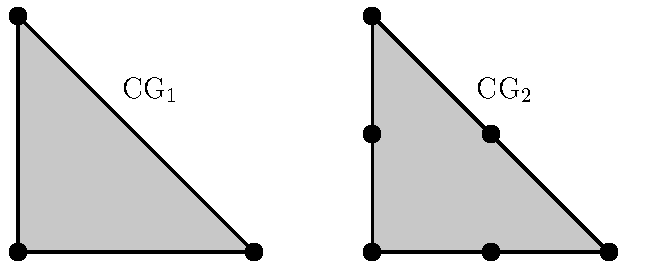
\includegraphics[width=0.6\linewidth]{./figures/eulerian/continuousGalerkin.pdf}
	\caption{The Lagrange $\mathrm{CG}_q$ triangle for $q = 1, 2$. The triangles have $3$ and $6$ DOFs respectively ({\color{black}{$\bullet$}}, black dot).}
	\label{fig:continuousGalerkin}
	\end{figure}



\subsection*{Variational formulation}
\label{subsec:variationalProblem}

To solve a basic problem such as a Poisson equation numerically, we need to convert it into a variational problem. The methodology is followed from the \fenics tutorial provide by Langtangen \cite{Logg2012b}. A 1D Poisson problem is given as,
	\begin{equation}
	\begin{aligned}
	- \nabla^2 u(x) &= f(x), \qquad x\ \mathrm{in}\ \Omega,\\
	u(x) &= u_0(x), \qquad x\ \mathrm{on}\ \partial\Omega.
	\end{aligned}
	\label{eq:poissonEq}
	\end{equation}
	
We can transform equation \ref{eq:poissonEq} into a variational form by multiplying it with a test function $v$, and integrating it over the domain $\Omega$,
	\begin{equation}
	- \int_{\Omega} \left(\nabla^2 u\right)v\ \mathrm{d}x= \int_{\Omega} fv\ \mathrm{d}x, \qquad \forall\ v \in \hat{V}.
	\label{eq:poissonEqVariationFormA}
	\end{equation}

In variational form equation \ref{eq:poissonEqVariationFormA}, the function $u$ is known as the trial function, and is what we are trying to approximate. The trial function $u$ lies in the trial function space $V$, and the test function $v$ lies in the test function space $\hat{V}$. When performing integration by parts, the test function $v$ is required to be zero at regions where $u$ is known. So, the additional terms cancel and we get,

	\begin{equation}
	- \int_{\Omega} \nabla u \nabla v\ \mathrm{d}x= \int_{\Omega} fv\ \mathrm{d}x \qquad \forall\ v \in \hat{V}
	\label{eq:poissonEqVariationFormB}
	\end{equation}

This form is referred to as the ``weak-form" of the original Poisson equation and is valid for all $v$ in the trial space $\hat{V}$. An inner product of any two function $f$ and $g$ in domain $Omega$ is defined as,
	\begin{equation}
	\langle f,g \rangle = \int_{\Omega}fg\ \mathrm{d}x,
	\end{equation}
so we can simplify equation \ref{eq:poissonEqVariationFormB} to,
	\begin{equation}
	\langle \nabla u,\nabla v \rangle = \langle f,v \rangle, \qquad \forall\ v \in \hat{V}.
	\end{equation}

In order to solve this continuous problem numerically, we must transform it into discrete variational problem,

	\begin{equation}
	-\langle \nabla u_h, \nabla v \rangle = \langle f, v \rangle \qquad \forall\ v \in \hat{V}_h \subset \hat{V},
	\label{eq:poissonEqDiscreteVariational}
	\end{equation}

where $u_h$ is the discrete function in the discrete space $V_h$ which is a subset of $V$, and the discrete function space $\hat{V}_h$ is a subset of $\hat{V}$. A common choice for the function space is linear triangular element with three nodes (Courant triangle), as shown in figure \ref{fig:continuousGalerkin}, where $\hat{V}_h$ and $V_h$ are described by piecewise linear functions of the triangle. At the boundary, the functions in the test space is zero, whereas the functions in the trial space is equal the boundary condition $u_0$.  The equation \ref{eq:poissonEqDiscreteVariational} can be simplified as,
	\begin{equation}
	a\left(u,v\right) = L(v),
	\label{eq:weakForm}
	\end{equation}
where,
	\begin{equation}
	a\left(u,v\right) = - \langle \nabla u, \nabla v \rangle,
	\end{equation}
and
	\begin{equation}
	L(v) = \langle f,v \rangle.
	\end{equation}

The variable $a(u,v)$ and $L(v)$ is the denoted as the bilinear and linear form, respectively. For simplicity, we will ignore the discrete notation (i.e $\{\cdot\}_h \rightarrow \{\cdot\}$). To solve for the discrete solution we substitute,	
	\begin{equation}
	u = \sum_{j=1}^{N} U_j \phi_j,
	\label{eq:trialDiscrete}
	\end{equation}
the linear combination of the basis function $\phi_j$, spanning the function space $V$, into $a\left(u,v\right)$. The test function is linear combination of the basis function $\hat{\phi}_i$, spanning the test space $\hat{V}$, which is defined as
	\begin{equation}
	v=\sum_{i=1}^{N} \hat{\phi}_i.
	\label{eq:testDiscrete}
	\end{equation}
	
The test function $v$ is taken to be zero at the boundary and one everywhere else. Substituting equation \ref{eq:trialDiscrete} and \ref{eq:testDiscrete} into equation \ref{eq:weakForm} gives,
	
	\begin{equation}
	\sum_{j=1}^N a(\phi,\hat{\phi}_i)\ U_j = L(\hat{\phi}_i).
	\end{equation}

Thus, we have to solve a linear system of equations given as,

	\begin{equation}
	\mathbf{A}U = b,
	\label{eq:linearSysOfEq}
	\end{equation}	
	
where $\mathbf{A}_{ij} = a(\phi_j,\hat{\phi}_i)$ is the coefficient matrix, and $b$ is the \printAcron{Right-Hand Side}{RHS} containing the knowns of the problem.
 	
%------------------------------------------------------------------------------------------------------
%------------------------------------------------------------------------------------------------------
%------------------------------------------------------------------------------------------------------
\section{Solving the Finite Element problem}

To solve this linear system of equations, equation \ref{eq:linearSysOfEq}, we used the \fenics Project that had implemented a comprehensive library of finite elements,, high performance linear algebra, and a scripting interface in \textsc{Python}. The scripting interface in \python enabled us to perform computation similar to a \matlab interface, where we could focus on the development of the algorithm, with minimal time spend on the code generation and the debugging process. The \dolfin library from the \fenics Project was used in python to define the finite element problem. 

In order to generate the mesh of the fluid domain, we used \gmsh, a three-dimensional finite element mesh generator which proves a fast, light and user-friendly meshing tools.

\subsection{Introduction to FEniCS Project}

The \fenics Project is a collaborative work of various universities, that developed tools to perform automated finite element algorithms that can be used to solve the solutions of the partial differential equation. It was a project originated in 2003 with the research collaboration of University of Chicago and Chalmers University of Technology with Logg,  Mardal, and Wells \cite{Logg2012b}. Since then, it has been expanded to various institutes such as Royal Institute of Technology, Simula Research Laboratory, University of Cambridge, and Delft University of Technology.

	\begin{figure}[p]
	\centering
	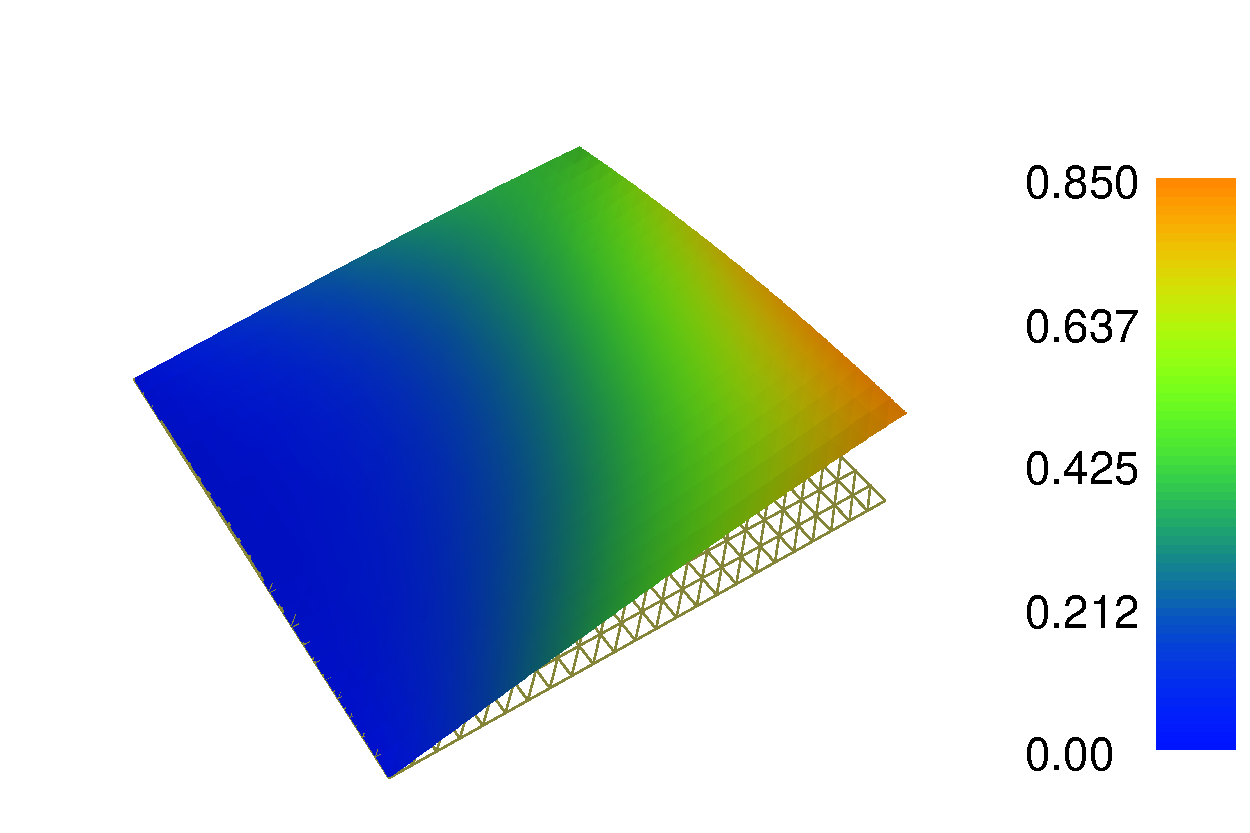
\includegraphics[width=0.5\linewidth]{./figures/eulerian/dolfinExampleFigure-rotated270.pdf}
	\caption{\dolfin VTK plot of the Poisson solution, given by the problem, source code listing \ref{lst:pycode-poisson}.}
	\label{fig:dolfinExampleFigure}
	\end{figure}

	\begin{listing}[p]
	\inputminted[fontseries=courier,obeytabs,fontsize=\footnotesize,mathescape,linenos,numbersep=5pt,frame=lines,framesep=2mm,xleftmargin=20mm,xrightmargin=20mm]{python}{figures/eulerian/dolfinExample.py}
	\caption{A complete program for solving the Poisson problem and plotting the solution. The Poisson problem is given as $-\nabla^2{u} = f$, where $u_0 = \sin{x}\cdot\cos{y}$ on the boundary and $f=2$. The code is written in \python using \dolfin 1.2 library}
	\label{lst:pycode-poisson}
	\end{listing}

The consists of various libraries such as UFC, UFL, FIAT, INSTANT and mainly \textsc{Dolfin}. \dolfin is the core library aimed at automating the solution of partial differential equations using finite element method \cite{Logg2010a}. It uses automated code generation maintaining high level of mathematical expressions and internally providing efficient, multi-threaded performance using the \indexAcron{Message Passing Interface}{MPI}. It used built-in linear algebra backend such as PETSc, TRILINOS/EPECTRA, uBLAS, and MTL4.

We used the \dolfin library in \python to solve the Poisson problem, equation \ref{eq:poissonEq}. We took $f=2$ and,
	\begin{equation}
	u(x) = u_0(x) = \sin x \cdot \cos y,
	\end{equation}
on boundary $\partial \Omega$. The code generation of the finite element was automated with the \dolfin library, leaving only the explicit expression of the problem in python. The source code to the Poisson problem is listed in listing \ref{lst:pycode-poisson}, and we see that it is a direct explicit translation of the problem, with small overheads of constructing the finite element problem.

\subsection{Mesh generation using GMSH}

The proper generation of the fluid mesh is an important aspect of the Finite Element method. It is an important process, as an ill-construct mesh can be computationally very expensive, or might even problem with convergence. There have been literatures dedicated just to improve the mesh generation, for example by Hansen \cite{Hansen2005}. It focused on mesh enhancement techniques for elliptical methods, which enables to increase the quality of the data, and also the robustness of the simulation.

For the generation of the mesh, we use \gmsh, an open-source software developed by Geuzaine and Remacle \cite{Geuzaine2009b}, which has implemented a user-friendly interface and fast algorithms. The \gmsh implemented kernels that use \textsc{BLAS} and LAPACK linear algebra packages in C++ for fast computation. Furthermore, it allows for scriptability making it ideal to integrate it with our current \python code project for future automation.

\section{Solving Incompressible Navier-Stokes Equations}
The finite element method will be used to describe the Eulerian domain of the hybrid scheme. In the Lagrangian domain, we have used the vorticity-velocity $\omega-\mathbf{u}$ formulation of the Navier-Stokes to describe the evolution of the vorticity in the wake. However, in the Eulerian domain, we will use the primitive variables, the velocity-pressure $\mathbf{u}-p$ formulation of the fluid, so that we can directly enforce the no-slip Dirichlet velocity boundary condition at the wall of the body. 

\subsection{Velocity-pressure formulation}
The velocity-pressure $\mathbf{u}-p$ formulation of the fluid, is the standard formulation of the Navier-Stokes equations of the fluid dynamics problem. The 2-D incompressible Navier-Stokes equations of a fluid with unit density (i.e $\rho = 1$) is given as,
	\begin{subequations}
	\begin{align}
	\frac{\partial \mathbf{u}}{\partial t} + \mathbf{u}\cdot\nabla\mathbf{u} - \nabla \cdot \sigma &= f,\\
	\nabla \cdot \mathbf{u} = 0,
	\end{align}	
	\label{eq:2Dns}
	\end{subequations}
where $\sigma$ is the Cauchy stress tensor defined as,
	\begin{equation}
	\sigma(\mathbf{u},p) = 2\nu\epsilon(\mathbf{u}) - p\mathbf{I}.
	\end{equation}

The Cauchy stress tensor is a function of pressure $p$, the fluid kinematic viscosity $\nu$, and the symmetric gradient $\epsilon$,
	\begin{equation}
	\epsilon(\mathbf{u}) = \frac{1}{2} \left(\nabla \mathbf{u} + \nabla \mathbf{u}^{\mathrm{T}}\right).
	\label{eq:symGrad}
	\end{equation}

So the Cauchy stress tensor defines the stress at a point in fluid due to the velocity gradient and the pressure. The incompressible 2-D Navier-Stokes equations have two unknowns, the vector velocity field $\mathbf{u}$, that lies on the vector-valued function space $V$, and the scalar pressure field $p$, which lies on the scalar-valued function space $Q$. Onces we solve for both these primitive variables, we can transfer this solution on the Lagrangian domain using the hybrid scheme. The hybrid scheme that we employ for this research, requires the transfer of the vorticity field from the Eulerian domain (i.e Eulerian grid), onto the vortex particles of the Lagrangian domain.


\subsection{Determining the vorticity field}

	\begin{listing}[t]
	\inputminted[fontseries=courier,obeytabs,fontsize=\footnotesize,mathescape,linenos,numbersep=5pt,frame=lines,framesep=2mm,xleftmargin=20mm,xrightmargin=20mm]{python}{figures/eulerian/vorticity.py}
	\caption{The \textsc{python} implementation of the vorticity calculation}
	\label{lst:pycode-vorticity}
	\end{listing}

The coupling between the Eulerian to Lagrangian method is through the transfer of the vorticity field $\omega$ from the Eulerian domain to the Lagrangian vortex blobs. The vorticity field $\omega$, is defined as,

	\begin{equation}
	\omega = \nabla \times u,
	\label{eq:vorticityEq}
	\end{equation}

and is defined as the curl of the velocity field $\mathbf{u}$. The vorticity field $\omega$ is  a scalar field that lies on the scalar-valued function space $W$. As the velocity field changes every at time $t_n$, we will have to evaluate the curl of the velocity at every step, $t_n, t_{n+1}, ...$. This brings the need for calculating the vorticity in an efficient manner, as we should not have to reconstruct the problem every step. To solve this problem in a efficient manner, \textsc{FEniCS} has implemented a function that can pre-assemble (i.e pre-calculate) the fixed parameters of the problem. To do this, we must first define equation \ref{eq:vorticityEq} in the variational (integral) form,  
	\begin{equation}
	\int_{\Omega} \omega \cdot \mathbf{v}\ \mathrm{d}x = \int_{\Omega} (\nabla \times \mathbf{u},) \cdot \mathbf{v}\ \mathrm{d}x,
	\end{equation}
where $\omega = \sum_{j=1}^N \hat{\omega}_j\psi_j$, is a linear combination of basis function $\psi_j$, spanning the function space $W$. The variational form is summarized as
	\begin{equation}
	a(\omega,\mathbf{v}) = L(\mathbf{u},\mathbf{v})
	\end{equation}
where $a(\omega,v)$ contains the knowns of the problem, which are fixed during the simulation. This can be pre-calculated to optimize the problem. $(\mathbf{u},\mathbf{v})$ is the unknown of the problem which has to be recalculated every time as it is a function of the current velocity. The \textsc{python} implementation of the algorithm is show in listing \ref{lst:pycode-vorticity}. Using the \dolfin library, we can used the \texttt{assemble} function to pre-calculated the LHS of the problem (line 10). So using the algorithms of the hybrid coupling scheme, we can transfer this vorticity field of the Eulerian domain on the vortex blobs.

\subsection{Taylor-Hood finite element family for solving ICNS}
To solve the \indexAcron{Incompressible Navier-Stokes}{ICNS} problem, we must choose an appropriate finite element function spaces for the velocity $\mathbf{u}$, the pressure $p$, and the vorticity. When determining proper mix of finite elements, we have to ensure that it satisfies the Ladyzhenskaya-Babu\v{s}ka-Brezzi (LBB) compatibility condition, also known as the inf-sup compatibility condition \cite{Brezzi1991}. When using the Lagrange finite element spaces, we have to ensure that the order of the velocity $q_{\mathrm{vel}}$, is one order higher than the order of the pressure $q_{\mathrm{pres}}$,
	\begin{equation}
	q_{\mathrm{vel}} = 	q_{\mathrm{pres}} + 1.
	\end{equation}
Brezzi and Fortin \cite{Brezzi1991} showed that if both are of same order, it will result to an unstable problem. To solve the ICNS problem, we will used the Taylor-Hood family \cite{Taylor1973}, examined by Boffi \cite{Boffi1997}. The method use velocity order $q_{\mathrm{vel}} = 2$ and pressure order $q_{\mathrm{pres}} = 1$. We decided to choose this method, as it is the most conventional method, that is simple, and that shows a stable behavior.

In addition, we have to choose an appropriate function space for the vorticity field $\Omega$. As vorticity is the curl of the velocity, to reduce interpolation error during the projection of the solution, we will used function space one order lower than the velocity, $q_{\mathrm{vort}} = 1$. Table \ref{tab:eulerianFunctionTerms} shows the list of the function spaces, the finite element type and the order. In additional, we have included the variable names of the function space, trial functions and the test functions, associated to the function element that we have chosen for the problem.

	\ctable[
	    caption = {Summary of the Lagrange element $\mathrm{CG}_q$ of order $q$, that was used for solving the incompressible Navier-Stokes problem. The variable names of the function space, the trial functions, and the test functions are also tabulated together.},
	    label   = {tab:eulerianFunctionTerms},
	    pos = b,
	]{lcccc}{}{\FL
	Variable	& Finite element & Function space	& Trial function & Test function \ML
	Velocity	& $\mathrm{CG}_2$	& $V$			& $\mathbf{u}$	 & $\mathbf{v}$\\
	Pressure 	& $\mathrm{CG}_1$ 	& $Q$			& $p$	 		 & $q$\\
	Vorticity 	& $\mathrm{CG}_1$	& $X$			& $w$	 		 & $x$\LL}


\subsection{Incremental pressure correction scheme}

The algorithm to solve the Navier-Stokes problem was first demonstrated by Chorin in 1968 \cite{Chorin1968}, referred to as the Chorin's projection method or sometimes known as the non-incremental pressure correction scheme. The process relied on first computing a tentative velocity by initially neglecting the pressure in the momentum equation of the Navier-Stokes problem, equation \ref{eq:2Dns}. The velocity field is corrected by determining the pressure field satisfying a divergence free vector field. This method however does not satisfy the discrete incompressibility constraint exactly and so, Goda in 1979 \cite{Goda1979a}, introduced an improved \indexAcron{Incremental Pressure Correction Scheme}{IPCS}. The method computed the viscous term at the incremented time $(t_{n-1} + t_n)/2$, and used the stress formulation to determine the corrected pressure \cite{Logg2012b}. 

The detailed algorithms to the IPCS scheme, as demonstrated by the \fenics Project \cite{Logg2012b}, can be summarized as follows:

	\begin{enumerate}
	\item \textbf{Compute the tentative velocity:} The tentative velocity $\mathbf{u}^{\star}$ is determined by solving,
		\begin{equation}
		\begin{split}
		\langle D_t^n \mathbf{u}^{\star}, \mathbf{v} \rangle &+ \langle \mathbf{u}^{n-1}\cdot\nabla\mathbf{u}^{n-1},\mathbf{v}\rangle + \langle \sigma(\mathbf{u}^{n-\frac{1}{2}},p^{n-1}), \epsilon(\mathbf{v}) \rangle \quad \\ &\quad+ \langle p^{n-1}\hat{\mathbf{n}},\mathbf{v}\rangle_{\partial \Omega} - \langle \mathbf{v}\ \hat{\mathbf{n}} \cdot (\nabla \mathbf{u}^{n-\frac{1}{2}} )^{\mathrm{T}},\mathbf{v} \rangle_{\partial \Omega} = \langle f^n,\mathbf{v} \rangle,
		\end{split}
		\label{eq:tentativeVel}
		\end{equation}
	is valid for all $\mathbf{v} \in V$, where $\mathbf{u}^{n-\frac{1}{2}}$ is defined as,
		\begin{equation}
		\mathbf{u}^{n-\frac{1}{2}} = \frac{\mathbf{u}^{\star}+\mathbf{u}^{n-1}}{2},
		\end{equation}
	With the Dirichlet velocity boundary conditions at the boundary $\partial \Omega$, we can solve the equation \ref{eq:tentativeVel}. The additional term,
		\begin{equation}
		\langle \mathbf{v}\ \hat{\mathbf{n}} \cdot (\nabla \mathbf{u}^{n-\frac{1}{2}} )^{\mathrm{T}},\mathbf{v} \rangle_{\partial \Omega},
		\end{equation}
	is resulted from the integration by parts, when we evaluate the viscous term at $(t_{n-1} + t_n)/2$ and we use the stress formulation instead of the Laplacian formulation as done for the Chorin scheme. This difference ensures that the velocity profile at the inlet and the outlet of the domain is more accurate that the ones obtained for the Chorin scheme. 
	
	The source code for solving the tentative velocity problem is shown in listing \ref{lst:pycode-tentativeVelocity}. First, we pre-define all the terms need for the tentative velocity problem formulation (lines \numrange{3}{16}). We can also pre-assemble the LHS of the problem (line 19) outside of the time-integration loop, as it remains constant. During the time integration, we first assemble the RHS of the problem (line 26), then apply the Dirichlet velocity boundary condition (line 29) which consist of the wall boundary condition, and external Dirichlet velocity boundary condition (e.g. the free-stream). Finally, we can solve the problem using GMRES solver for solving the system of linear equations.
	
		\begin{listing}[t]
		\inputminted[fontseries=courier,obeytabs,fontsize=\scriptsize,mathescape,linenos,numbersep=5pt,frame=lines,framesep=2mm,xleftmargin=20mm,xrightmargin=20mm]{python}{figures/eulerian/tentativeVelocity.py}
		\caption{The source code for solving the tentative velocity $\mathbf{u}^{\star}$, using the equation \ref{eq:tentativeVel}}
		\label{lst:pycode-tentativeVelocity}
		\end{listing}
	
	\item \textbf{Determine the corrected pressure:} The corrected pressure $p^n$ is determined by solving,	
		\begin{equation}
		\langle \nabla p^n, \nabla q \rangle = \langle \nabla p^{n-1}, \nabla q\rangle - \langle \nabla \cdot \mathbf{u}^{\star}, q \rangle / \Delta t_n
		\label{eq:pressureCorrection}
		\end{equation}
	is valid for all $q \in Q$. We use the previously calculated tentative velocity $\mathbf{u}^{\star}$ to determine the corrected pressure. We can solve the problem using the Neumann pressure boundary condition at the pressure outlet of the domain. We define a boundary as the pressure outlet, if we do not know the velocity boundary condition at that boundary. This is true for the region were the exit flow is perturbed. However, for the coupled Eulerian method (that we will use), all the boundary conditions are available as a velocity boundary condition from the Lagrangian domain. This means that do not have to assume any pressure boundary condition.

	The source code for solving the  corrected pressure problem is shown in listing \ref{lst:pycode-correctedPressure}. As done for the tentative velocity, we formulate and pre-assemble the problems before the time loop. In the time loop, we only need to assemble the RHS, apply the boundary condition (if it exists), and finally solve for the corrected pressure. Using the corrected pressure, we can determine the corrected velocity field. 
		
		\begin{listing}[p]
		\inputminted[fontseries=courier,obeytabs,fontsize=\scriptsize,mathescape,linenos,numbersep=5pt,frame=lines,framesep=2mm,xleftmargin=20mm,xrightmargin=20mm]{python}{figures/eulerian/correctedPressure.py}
		\caption{The source code for solving the corrected pressure $p^n$ using the equation \ref{eq:pressureCorrection}}
		\label{lst:pycode-correctedPressure}
		\end{listing}
			
	\item \textbf{Determine the corrected velocity:} The corrected velocity field $u^n$ is determined by solving,
		\begin{equation}
		\langle \mathbf{u}^n, \mathbf{v}\rangle = \langle \mathbf{u}^{\star},\mathbf{v} \rangle - \Delta t_n \langle \nabla(p^n - p^{n-1}),\mathbf{v} \rangle,
		\end{equation}
	which is valid for all $\mathbf{v} \in V$. We correct the tentative velocity $\mathbf{u}^{\star}$ by the pressure difference to determine the correct velocity field. We will have to apply the Dirichlet velocity boundary condition at the boundary again, to solve for the problem.
	
	The source code of the solving the corrected pressure problem in shown in listing \ref{lst:pycode-correctedVelocity}.
	We first initialize the problem, by formulating the problem and assembling the LHS outside the time loop (line \numrange{3}{8}). In the time integration loop, we assemble the RHS, apply the velocity boundary condition and finally solve for the corrected velocity field.
	
		\begin{listing}[p]
		\inputminted[fontseries=courier,obeytabs,fontsize=\scriptsize,mathescape,linenos,numbersep=5pt,frame=lines,framesep=2mm,xleftmargin=20mm,xrightmargin=20mm]{python}{figures/eulerian/correctedVelocity.py}
		\caption{The source code for solving the corrected pressure $p^n$ using the equation \ref{eq:pressureCorrection}}
		\label{lst:pycode-correctedVelocity}
		\end{listing}
		
	\end{enumerate}
	
This algorithm was implemented using \textsc{Dolfin}'s Krylov \textsc{Gmres} solver with absolute and relative error tolerance of \num{e-25} and \num{e-12} respectively. The program structure was based on the collection of benchmark and solvers provided by the \fenics examples scripts \cite{nsbench}. The algorithm described above an explicit time marching scheme, also referred to as \indexAcron{Forward Euler}{FE}, which is the simplest time marching scheme. Therefore, for the time marching scheme to be stable, we require the CFL number satisfy the following condition:
	\begin{equation}
	\mathrm{CFL} = \Delta t_{\mathrm{max}} \frac{\lVert\mathbf{u}\rVert_{\mathrm{max}}(\nu +  \Delta h_{\mathrm{min}}\lVert\mathbf{u}\rVert_{\mathrm{max}})}{\Delta h_{\mathrm{min}}^2} \le 1.
	\label{eq:cfl}
	\end{equation}
	
	\begin{figure}[t]
	\centering
	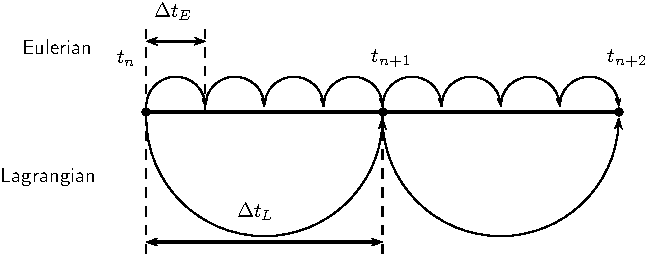
\includegraphics[width=0.7\linewidth]{./figures/eulerian/multiStep-crop.pdf}
	\caption{Eulerian multi-stepping to match the lagrangian $\Delta t_L$. The figures shows $\Delta t_L = 4 \Delta t_E$ and required $k_E = 4$ iterations to time march from $t_n$ to $t_{n+1}$.}
	\label{fig:multiStep}
	\end{figure}		
	
This gives us the direct constraint on the maximum Eulerian time step size $\Delta t_{E,\mathrm{max}}$ which is function of the $\mathrm{CFL}$ number, maximum fluid velocity in the Eulerian domain $\lVert \mathbf{u} \rVert_{\mathrm{max}}$, the fluid viscosity $\nu$ and the minimum mesh cell size $\Delta h_{min}$. When coupling with the Lagrangian method, we will see that $\Delta t_E \le \Delta t_L$ (Lagrangian time step size is ideally larger than Eulerian time step size), meaning that we will have to perform $k_E$ Eulerian sub-steps to reach the Lagrangian step, figure \ref{fig:multiStep}.

\subsection{Determining the body forces}

	\begin{listing}[t]
	\inputminted[fontseries=courier,obeytabs,fontsize=\footnotesize,mathescape,linenos,numbersep=5pt,frame=lines,framesep=2mm,xleftmargin=20mm,xrightmargin=20mm]{python}{figures/eulerian/forces.py}
	\caption{The \textsc{python} implementation of the force calculation}
	\label{lst:pycode-forceCalculation}
	\end{listing}

Once we solved for flow fields, it is a common strategy to verify the results using some sort of quantities. In aerodynamics, (especially in aerospace field), we like the evaluated the lift and drag coefficient of a given geometry and compare the results to available literature. In order to determine these coefficient, we must first determines the 
friction force and the pressure force acting on the no-slip boundary, or simply put, it is the total stress tensor $\sigma$ acting on the surface of the body. The stress tensor $\sigma$ is given by
	\begin{equation}
	\sigma(\mathbf{u},p) = 2\nu\epsilon(\mathbf{u}) - p\mathbf{I},
	\end{equation}
where $\epsilon$ is the symmetric gradient, equation \ref{eq:symGrad}, and is a function of the velocity $\mathbf{u}$ and the pressure $p$ acting on the surface.The lift coefficient and the drag coefficient is computed as,
	\begin{subequations}
	\begin{align}
	L &= \int_{\partial \Omega} \left[\sigma(\mathbf{u},p) \cdot \hat{\mathbf{n}}\right]\cdot \hat{\mathbf{e}}_y\ \mathrm{d}s,\\
	D &= \int_{\partial \Omega} \left[\sigma(\mathbf{u},p) \cdot \hat{\mathbf{n}}\right]\cdot \hat{\mathbf{e}}_x\ \mathrm{d}s,
	\end{align}
	\end{subequations}
where $\hat{\mathbf{e}}_x$ and $\hat{\mathbf{e}}_y$ are the 2D unit Cartesian vectors,
	\begin{equation}
	\hat{\mathbf{e}}_x = \begin{bmatrix}
	 1 \\ 
	 0 
	\end{bmatrix}, \qquad \quad 
	\hat{\mathbf{e}}_y = \begin{bmatrix}
		 0 \\ 
		 1 
		\end{bmatrix}.\\
	\end{equation}

The lift coefficient and the drag coefficient, $C_l$ and $C_d$ respectively, is the lift and drag normalized with the dynamics pressure and reference length $c$ (in 2D), where the lift perpendicular to the free-steam and the drag is tangential to it,
		\begin{equation}
		C_l = \frac{L}{\frac{1}{2}\lVert\mathbf{u}\rVert_{\infty}^2 c},\qquad \quad
		C_d = \frac{D}{\frac{1}{2}\lVert\mathbf{u}\rVert_{\infty}^2 c}.\\
		\end{equation}


%		\begin{subequations}
%		\begin{align}
%		C_l &= \frac{L}{\frac{1}{2}\lVert\mathbf{u}\rVert_{\infty}^2 c},\\
%		C_d &= \frac{D}{\frac{1}{2}\lVert\mathbf{u}\rVert_{\infty}^2 c}.
%		\end{align}
%		\end{subequations}

\section{Validation of eulerian method}
To validate our Eulerian method, we will first investigate the problem of the Lamb-Oseen vortex. Then we will compare the results of the Clercx-Bruneau dipole collison at $Re=625$. Finally, we will investigate the problem of the Impulsively started cylinder at $Re=550$.

\subsection{Lamb-Oseen Vortex}

	\ctable[
		caption = {Summary of the parameters for the Lamb-Oseen vortex evolution.},
		label   = {tab:eulerianLambOseenParams},
		pos = t,]{lcll}{}{\FL
		
		Parameters 					& Value 	& Unit					& Description \ML
		$\Gamma_c$\T               	& 1 &\si{m^2.s^{-1}} 				& Core strength\\
		$\Omega$               		& $\left[-1,1\right]^2$ &\si{m}		& Eulerian domain bounds \\
		$\mathbf{u}_{\infty}$ 		& $\left[0, 0\right]$ &\si{m.s^{-1}} & Free-stream velocity\\
		$\nu$						& $\num{5e-4}$ &\si{kg.s^{-1}.m^{-1}}& Kinematic viscosity\\
		$ (\tau_0,\tau_f)$ 		    & \numrange{2e-3}{2.5e-3} &\si{m^2}	& Initial and final scaled viscous time\\
		$ (t_0,t_f)$ 		    	& \numrange{4}{5} &\si{s}			& Initial and final simulation time\\		
		$ h_{\mathrm{min}}$			& $\frac{1}{100}\sqrt{2}$ &\si{m}			& Minimum mesh cell size\\	        
		$ N_{\mathrm{cells}}$ 		& $200^2$ 	& -						& Number of mesh cells\\
		$ \mathrm{CFL}$								& $0.95$ & -		& CFL number\\	        	        
		$\lVert \mathbf{u} \rVert_{\mathrm{max}}$	& $1.5$	& 	\si{m.s^{-1}} & Maximum magnitude fo the velocity\\		
		$ \Delta t$ 				& $0.001$ &\si{s}					& Time step size\\
		$ N_{\mathrm{t-steps}}$ 	& 1000 & -							& Number of time integration steps\\
		$\mathrm{ID}_{\mathrm{fluid}}$ & $1$ & - & Fluid domain I.D\\
		$\mathrm{ID}_{\mathrm{ext}}$ & $3$ & - & External Dirichlet velocity boundary I.D\LL}

The Lamb-Oseen vortex is an analytical solution by Lamb and Oseen, describing the diffusion of a vortex core \cite{Tryggeson2007}. We solved the same problem as the one described in the Lagrangian validation problem \ref{subsec:lagrangianLambOseen}. However, Eulerian domain use the primitive variables $\mathbf{u}-p$ for formulating the problem. Therefore, the initial conditions of the problem was the velocity field of Lamb-Oseen vortex,
	\begin{subequations}
	\begin{align}
	u_{\theta} &= \frac{\Gamma_c}{2\pi r} \left[1-\exp\left(-\frac{r^2}{4\tau}\right)\right]\\
	u_r &= 0,
	\end{align}
	\end{subequations}
where $\Gamma_c$ is the vortex core strength, $\tau \equiv \nu t$ is the scaled viscous time, and $r$ is the distance from the core center. The parameters of the simulation is tabulated in table \ref{tab:eulerianLambOseenParams}. To make the Eulerian simulation comparable with the Lagrangian simulation, we tried to match the spatial discretization of the Eulerian domain with the Lagrangian domain. The figure \ref{fig:lambOseenDomainDefinition} shows the domain of the problem, discretized the domain $\Omega = \left[-1,1\right]^2$ in a structure grid with the number of finite element cells $N_{\mathrm{cells}}=200^2$ in $x$ and $y$ direction, minimum cell size $h=\sqrt{2}/100$. 

	\begin{figure}[t]
	\centering
	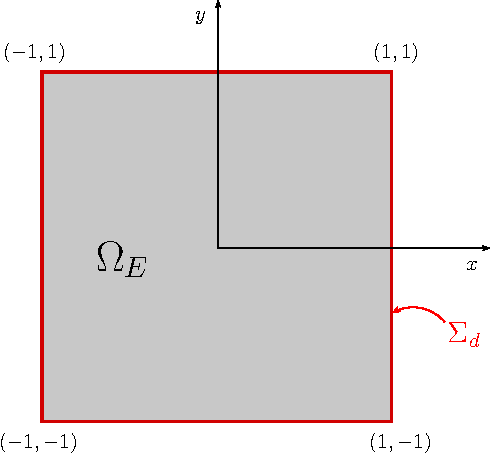
\includegraphics[width=0.5\linewidth]{./figures/eulerian/lambOseenDomainDefinition-crop.pdf}
	\caption{Eulerian domain for the Lamb-Oseen vortex problem. Figure shows the bound of the domain $\Omega = \left[-1,1\right]^2$, identified as $\mathrm{ID}_{\mathrm{fluid}} = 1$; and the boundary domain $\partial \Omega$ [{\color{plotRed}{---}}, solid red], identified as  $\mathrm{ID}_{\mathrm{ext}} = 3$, which is where the Dirichlet velocity boundary condition was applied.}
	\label{fig:lambOseenDomainDefinition}
	\end{figure}

Furthermore, the Figure \ref{fig:lambOseenDomainDefinition} also shows the boundary domains $\partial \Omega$ of the fluid domain. For the Lamb-Oseen problem, as we have the analytical solution of the velocity field for all time, we can use this solution to prescribe the external domain boundary condition. So for this problem, we only need an external Dirichlet velocity boundary condition, at the boundary domain identified as, $\mathrm{ID}_{\mathrm{ext}} = 3$. This would imply that we do not need to explicitly apply pressure boundary condition, as we already have a velocity boundary condition. With all the boundary conditions, we can evolve the initial velocity distribution of the Lamb-Oseen vortex from $t_0 = 4$ to $t_f =5$, using the IPCS algorithm described in section \ref{sec}. 

	\begin{figure}[b]
	\centering
	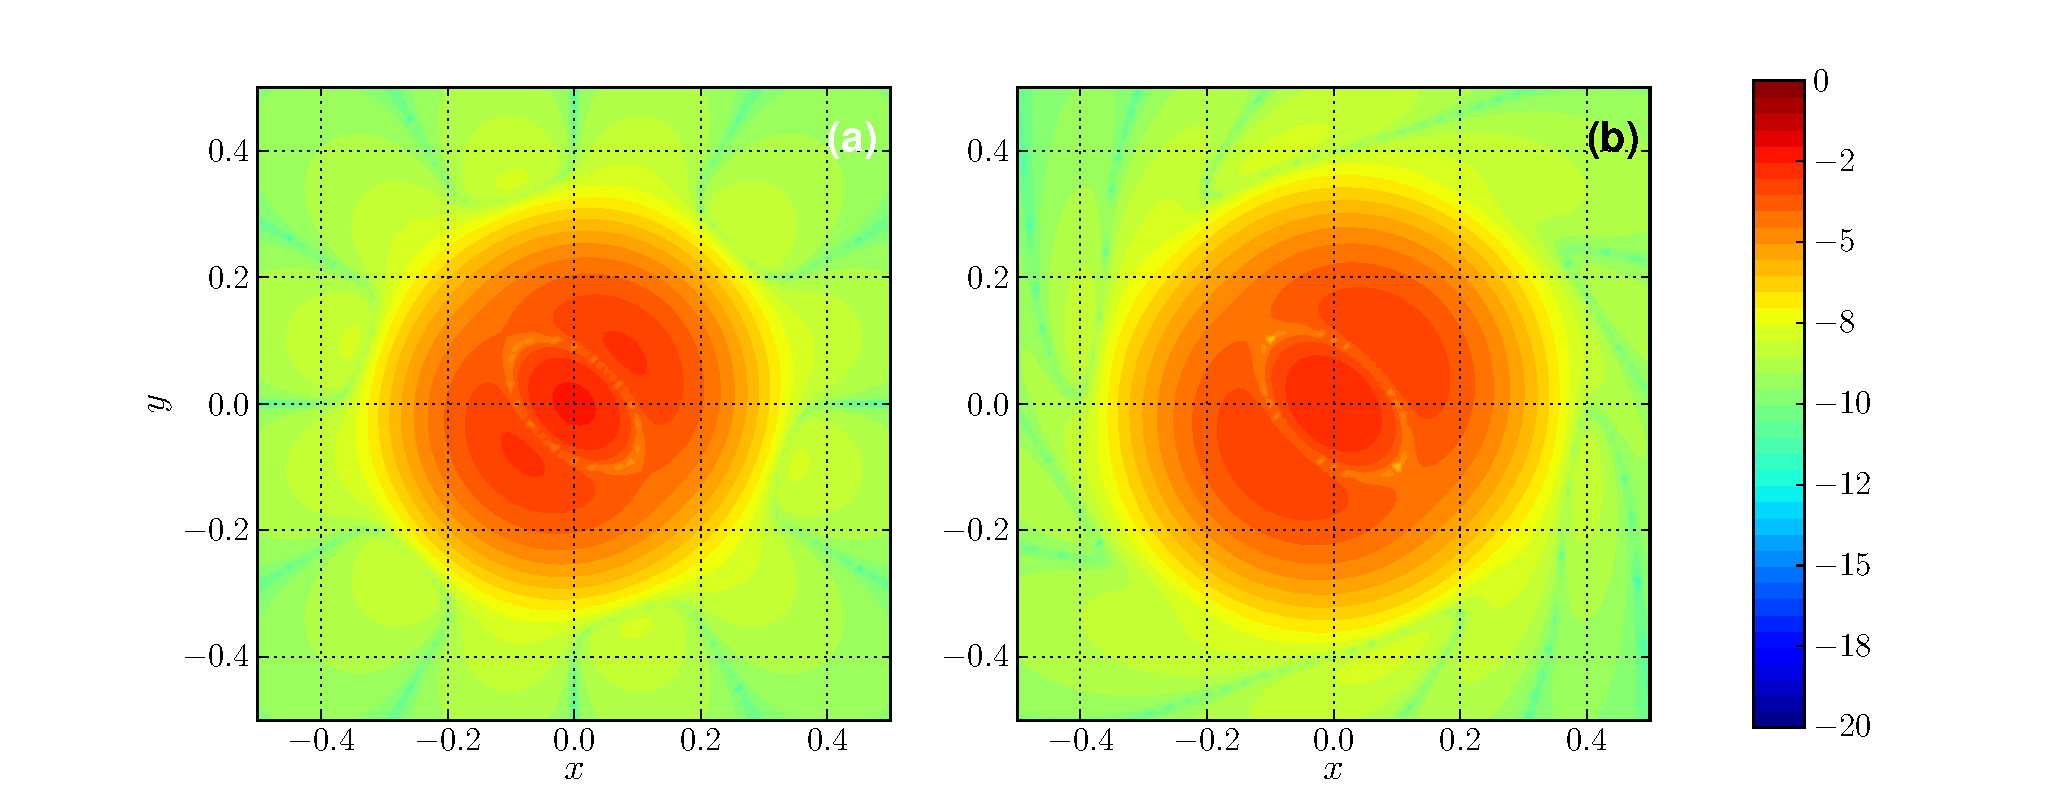
\includegraphics[width=0.8\linewidth]{./figures/eulerian/lambOseen_eulerian_wRelField_compressed.pdf}
	\caption{Relative error in vorticity field in logarithmic scale. Figure \textbf{(a)} shows the initial relative error in vorticity at $t=t_0$, and figure \textbf{(b)} shows the relative error in vorticity at the end of the time stepping $t=t_f$.}
	\label{fig:lambOseen_eulerian_wRelField_compressed}
	\end{figure}
	
We used $CFL$ stability condition equation \ref{eq:cfl}, to determine the time step size, $\Delta t = 0.001$. The Eulerian method time steps using a \printAcron{Forward Euler}{FE} time marching and requires $N_{\mathrm{t-steps}}=1000$ time steps. During the evolution, we evaluated the growth of the error in velocity, and in vorticity between the numerical results and the analytical solution. As mainly we are interested in the error in vorticity, as this is the quantity which will be interpolated onto the Lagrangian domain, figure \ref{fig:lambOseen_eulerian_wRelField_compressed} shows the initial and the final relative error in vorticity over the Eulerian domain. Opposed to the Lagrangian results, figure \ref{fig:lambOseen_convection_vorticityErrorContours_compressed}, we see that initial relative error in the vorticity field is larger. This is so because, the Lagrangian domain was initialized using the vorticity, where as the Eulerian domain was initialized using the velocity. To calculate the vorticity on the Eulerian domain, we had to project curl the velocity onto the function space of vorticity $W$. This process of initialization in the finite element domain and project of the vorticity introduced additional numerical error. However, the pattern of the relative error in vorticity, is similar to the Lagrangian solution, as the highest error is localized to the core center, where we have the highest gradient in vorticity.

	\begin{figure}[t]
	\centering
	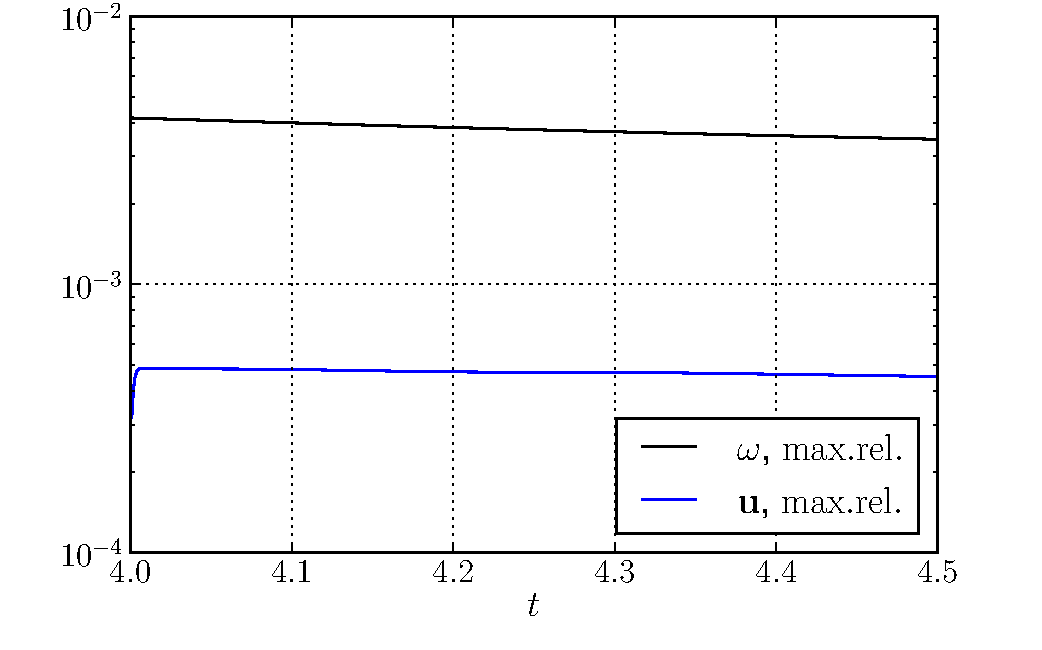
\includegraphics[width=0.7\linewidth]{./figures/eulerian/lambOseen_eulerian_wRelEvolution_compressed.pdf}
	\caption{Eulerian Lamb-Oseen relative vorticity evolution}
	\label{fig:lambOseen_eulerian_wRelEvolution}
	\end{figure}

	\begin{figure}[b]
        \centering
        \begin{subfigure}[b]{0.5\textwidth}
                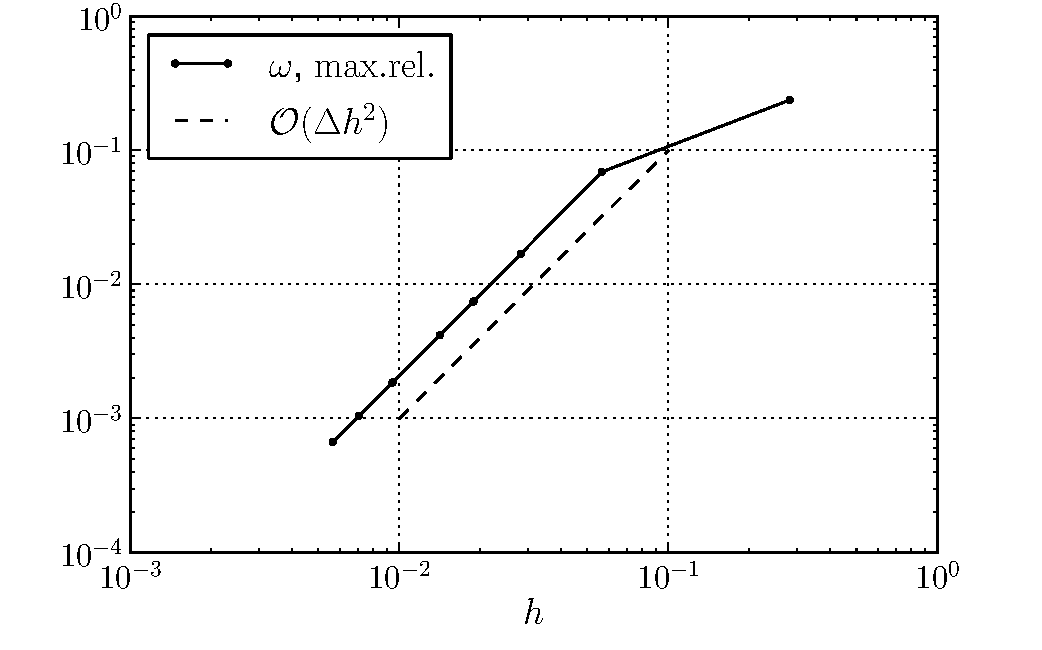
\includegraphics[width=\textwidth]{figures/eulerian/lambOseen_eulerianConvergence_dx_compressed.pdf}
                \caption{Lamb-Oseen dx convergence}
                \label{fig:lambOseen_eulerianConvergence_dx}
        \end{subfigure}%
        ~ %add desired spacing between images, e. g. ~, \quad, \qquad etc.
          %(or a blank line to force the subfigure onto a new line)
        \begin{subfigure}[b]{0.5\textwidth}
                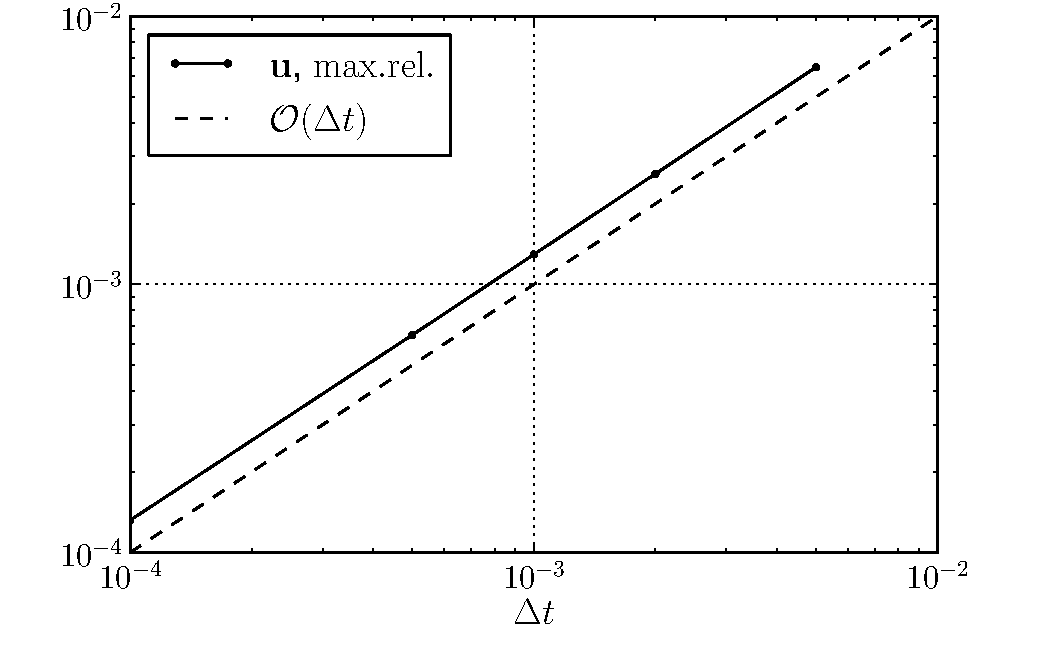
\includegraphics[width=\textwidth]{figures/eulerian/lambOseen_eulerianConvergence_dt_compressed.pdf}
                \caption{Lamb-Oseen dt convergence}
                \label{fig:lambOseen_eulerianConvergence_dt}
        \end{subfigure}
        \caption{Lamb-Oseen convergence}
        \label{fig:lambOseen_eulerianConvergence}
	\end{figure}	


As the time progress, we see that the error of the problem is stable and does not increase as observed for the Lagrangian domain, figure \ref{fig:lambOseen_eulerian_wRelField_compressed}b. The growth of the relative error in velocity and vorticity can be observed in figure \ref{fig: lambOseen_eulerian_wRelEvolution}. It shows that during the evolution of the Lamb-Oseen vortex, the relative error in velocity, and vorticity is stable. We see that due to the relation of vorticity to velocity, the error in vorticity is higher that velocity. However, the stability in the error of the solution is vital as it verifies that our method is stable and robust for solving the problem.

In order to have an extensive understanding of the stability of our scheme, we investigated the convergence of the spatial and temporal discretization of the domain. To determine the convergence of space, the simulation was run for $h \approx 0.25$ to $h \approx \num{5e-3}$. Figure \ref{fig:lambOseen_eulerianConvergence_dx} shows the convergence of the relative error in vorticity, due to increase in spatial resolution. This validates that the scheme is $2^{nd}$-order in space, due to second order function space $CG_2$ for the primitive variable, velocity.

To determine convergence in time, we ran the simulation with various time steps $\Delta t = \num{5e-3}$ to $\Delta t = \num{1e-4}$). As we performed the investigation, we saw that the error in primitive variable $\mathbf{u}$, converged at an order 1, figure \ref{fig:lambOseen_eulerianConvergence}. This is true to the theory, as we are employing a $1^{\mathrm{st}}$-order Forward Euler scheme for the time integration. Thus, we have verified with the analytical solution of the Lamb-Oseen vortex that our Eulerian method is implemented according to the theory, and perform in a robust manner.
	


\subsection{Clercx-Bruneau dipole collison at $Re=625$}
To validate that our Eulerian method performs according to theory, and to provide a benchmark case for the hybrid coupling scheme, we decided to simulate a flow where the generation of the vorticity from the wall is the main focus. To generate this benchmark case, we used the numerical experiment benchmarked by Clercx and Bruneu in 2005 \cite{}, on  the collison of the dipole with a no-slip boundary. 

The reason for using the Clercx-Bruneau dipole for validation is because, it a common practise to use the dipole-wall collision test case to validate the numerical method. Ould-salihi et al \cite{} used this case to validate their Hybrid method that couples vortex particles with finite-difference method. Cottet et al. \cite{} used the collision to tool to validate the vortex method.

Clercx and Bruneau have stated that dipole-wall interaction test cases are ideal for methods requiring the well-resolvedness of the thin boundary layer near the no-slip walls. The literature determined the convergence of the numerical solution by investigating quantities like the total kinetic energy, the enstrophy and the total angular momentum of the flow. It mainly focuses on the vorticity distribution and the vorticity flux at the no-slip boundary of the domain. Furthermore, this literature provided well-defined initial and boundary conditions, with smooth vorticity distribution as seen for the Lamb-Oseen vortex case.

The Clercx-Bruneau test case investiated the normal collision of a dipole with a no-slip wall. The parameters of the problem are tabulated in table \ref{tab}. 

	\ctable[
		caption = {Summary of the parameters for the Clercx-Bruneau normal collsion of a dipole with a no-slip wall \cite{}.},
		label   = {tab:clercxBruneauParameters},
		pos = t,]{lcll}{}{\FL
		
		Parameters 					& Value 				& Unit		& Description \ML
		
		$\Omega$               		& $\left[-1,1\right]^2$ &\si{m}		& Eulerian domain bounds \\
		$Re = UW/\nu$         		& $625$ 				&-			& Reynolds number \\
		$W$			         		& $1$ 					&\si{m}		& Half width of the domain\\		
		$U$			         		& $1$ 					&\si{m.s^{1}}& Characteristic velocity\\		
		$\nu$			         	& $1$ 					&\si{m.s^{1}}& Characteristic velocity\\			
		$\Gamma_c$\T               	& 1 &\si{m^2.s^{-1}} 				& Core strength\\

		$\mathbf{u}_{\infty}$ 		& $\left[0, 0\right]$ &\si{m.s^{-1}} & Free-stream velocity\\
		$\nu$						& $\num{5e-4}$ &\si{kg.s^{-1}.m^{-1}}& Kinematic viscosity\\
		$ (\tau_0,\tau_f)$ 		    & \numrange{2e-3}{2.5e-3} &\si{m^2}	& Initial and final scaled viscous time\\
		$ (t_0,t_f)$ 		    	& \numrange{4}{5} &\si{s}			& Initial and final simulation time\\		
		$ h_{\mathrm{min}}$			& $\frac{1}{100}\sqrt{2}$ &\si{m}			& Minimum mesh cell size\\	        
		$ N_{\mathrm{cells}}$ 		& $200^2$ 	& -						& Number of mesh cells\\
		$ \mathrm{CFL}$								& $0.95$ & -		& CFL number\\	        	        
		$\lVert \mathbf{u} \rVert_{\mathrm{max}}$	& $1.5$	& 	\si{m.s^{-1}} & Maximum magnitude fo the velocity\\		
		$ \Delta t$ 				& $0.001$ &\si{s}					& Time step size\\
		$ N_{\mathrm{t-steps}}$ 	& 1000 & -							& Number of time integration steps\\
		$\mathrm{ID}_{\mathrm{fluid}}$ & $1$ & - & Fluid domain I.D\\
		$\mathrm{ID}_{\mathrm{ext}}$ & $3$ & - & External Dirichlet velocity boundary I.D\LL}


The collison of a dipole normal to wall, from Clercx nand Bruneau \cite{}, was an ideal choice as the literature has provided a systematic methodology to perform the simulation and have provide detailed results.

The Clercx-Bruneau dipole

\subsection{Impulsively started cylinder at $Re=550$}

\section{Summary}

